\documentclass[uplatex,b5j,11pt]{jsbook}
\title{周期}

\usepackage[dvipdfmx]{graphicx}
\usepackage{fancybox}
\usepackage{amsmath,amssymb}
\usepackage{multicol}
\usepackage{ascmac}
\usepackage{booktabs}
\usepackage[dvipdfmx]{graphicx}
\usepackage[dvipdfmx]{color}
\usepackage{makeidx}
\usepackage{colortbl}
\usepackage{amsthm}
\usepackage{my-default}
\usepackage{tikz}


\begin{document}
\chapter{Introduction}
周期とは適当な関数を適切な範囲で積分したものである.
適当なの意味はものによって変わりうる.
ここではContesvich-Zagier予想や数論で出てくる周期に関する話ができればと思う.
自分の興味としては
\begin{itemize}
\item 計算との関連.
\begin{itemize}
  \item 計算可能実数や実閉体のモデル理論との関連.
  \item 数論的な対象が計算可能とは,どういう意味か?
\end{itemize}
\item 数論幾何的な対象の深い理解
\begin{itemize}
\item ドラムの定理との関連
\item モチーフ,数論的基本群との関連
\end{itemize}
\end{itemize}


%\chapter{リーマン面の理論}
\section{周期積分、ヤコビ多様体}
実際にリーマン面の理論の後半を読み,周期の関連を見る.

\subsection{位相幾何からの準備}
議論をする上で最低限のホモトピー論,ホモロジー論を定義する.
\begin{screen}
\begin{dfn}
 $X$上の2つの連続なpath $f,g: [0,1] \to X$に対し,連続写像$H:[0,1] \times [0,1] \to X$で
 $H(0, \cdot) = f(\cdot), H(1, \cdot)$となるものが存在するす時,$f,g$は\textbf{ホモトピック}という.
\end{dfn}
\end{screen}

\begin{screen}
\begin{dfn}
 $X$と$x \in X$に対して基点,つまり始点と終点が$x$となる連続なpath全体を$F$と表す.$\alpha, \beta \in F$に対して,
 \begin{equation*}
 \alpha \cdot \beta (t) = \begin{cases}
    \alpha(2t) & ( t \le 1/2) \\
    \beta(2t-1) & (t \ge 1/2)
  \end{cases}
 \end{equation*}
とすると,これは積構造を定める.
これをホモトピーによる同値関係で割ったものを\textbf{基本群}といい$\pi(X,x)$で表す.
すぐ計算すればわかるように,基本群上でも上で定めた積構造がwell-definedであり,この演算について群になる.
また,弧状連結である等,基点のとり方によらない場合は$\pi(X)$と表すこともある.
\end{dfn}
\end{screen}

\begin{screen}
\begin{dfn}
 $A \subset X$に対し,$F(x, 0) = x , F(x, 1) \in A , F(a, 1) = a$となる写像$F$を変位レトラクトという.
これは,$X$上の恒等写像と$A$へのレトラクション($A$への制限が恒等写像になるもの)の間のホモトピーの存在を意味する.
この時,$id$とレトラクトはホモトピー同値になる.ただし$A$に写像が制限されていないので,ホモトピー同値はホモトピックと同値になる.
\end{dfn}
\end{screen}

ホモロジー・コホモロジーについて定義する.
具体的な話を書きすぎると死んでしまうが,

\begin{itemize}
\item 特異ホモロジー
\item 単体ホモロジー
\item 特異コホモロジー
\item Kronecker積
\end{itemize}
について説明する.

$\Delta^n := \{ x \in \mathbb{R}^{n+1} \mid  \sum x_i =1, \forall x_i \ge 0 \}$とする.
$S_n(X) := \{f: \Delta^n \to X \mid f \mbox{は連続写像}\}$とし,
$C_n(X) := \oplus_{f \in S_n(X)} \mathbb{Z}$とする.
$i_j: \Delta_n \to \Delta_{n+1}$を第$j$成分を0にし,それ以降は一つずらしとする写像とする.
$d: S_n(X) \to S_{n-1}(X), \sum_{j} f \mapsto (-1)^j f \circ i_j$とする.
すると$d_n \circ d_{n+1} = 0$となり,

\begin{screen}
\begin{dfn}
$\mathcal{U} =  \{U_i\}_{i \in I}$を$X$の開被覆とする. 任意の有限個の$i_1, \ldots ,i_k \in I$に対し$ \cap U_i$が可縮な時,$\mathcal{U}$を\textbf{単純被覆}という.
$X$が$n$次元多様体であって,
\end{dfn}
\end{screen}

\subsection{ポアンカレの補題とドラムの定理}

%\chapter{GAGA}
GAGAでは射影代数多様上の層とそのanalyticなものが定めるコホモロジーの一致や圏同値を示す.
ここでは,最初にanalytic spaceとその上の層を定義する.
その後代数多様体に対し,代数多様体のanalytic化を定義し,射影代数多様体の場合の関係について示す.
\section{preliminary}
GAGAでは既知とされることを一定まとめておく.
ここでは層と環のflatについて説明する.
\subsection{sheaf}
GAGAでは層を普段とは異なる方法で定義しているため、その点に言及しておく.
GAGAやFACでは層を以下で定義している.
\begin{screen}
\begin{dfn}
\begin{itemize}
以下の組を層という.
  \item 位相空間$X$
  \item $x \in X$に対し,アーベル群$\mathcal{F}_x$が対応する.
  \item $\mathcal{F}$を集合としては$\mathcal{F}_x$のdisjoin unionとなる位相空間
\end{itemize}
$\pi: \mathcal{F} \to X$を$f \in \mathcal{F}_x$の時$\pi(f)=x$とする.
さらに
\begin{itemize}
  \item 任意の$f \in \mathcal{F}$に対し,$f \in \mathcal{F}$の近傍$V$と$\pi(f)=x$の近傍$W$で$V,W$が同相となるものが存在する.
  \item $f,g$に対し, $-f , f + g$がcontinuos(加法は$\pi(f) = \pi(g))$の時のみ.
\end{itemize}
\end{dfn}
\end{screen}

この時,$\Gamma(\mathcal{F}, U) := \{ s \in  \Hom_{conti}(U,\mathcal{F}) \mid \pi \circ s = id_u, \}$とすると,
これはアーベル群となる.
また,通常よくある層の公理を満たす.sectionなので明らかにわかる.非自明なのは連続性だけだが、貼り合わせを考えることでわかる.

逆にこちらの層を定義とする.
\begin{prop}
層の定義は互いに同値である.
\end{prop}
最初に$X, \mathcal{F}_x, \mathcal{F}, \pi$を定める.
$X$は元の位相空間のままとし,$\mathcal{F}_x := \varinjlim \mathcal{F}(U)$とする.$\mathcal{F}$は$\mathcal{F}_x$のdisjoint unionで定める.
$\mathcal{F}$の位相を定める.
$t \in \mathcal{F}(U)$と$x \in U$に対し,$\phi_x^U: \mathcal{F}(U) \to \mathcal{F}_x$とする.
$[t, U]$を$\{\phi_x^{U}(t)\}$のなす集合とする.
$\mathcal{F}$の$[t, U]$の生成する位相とする.実際にこの位相が局所同相性や演算の連続性を満たすことを示す.
実際$\phi_x^U(t)$の近傍として$[t,U]$がとれ,これは$U$と同相になる.
また,$f \mapsto -f$は$[t, U]$の逆像が,$[-t, U]$を対応させるのでのでcontinousであり,
$(f, g) \mapsto f + g$での$[t, U]$の逆像は
$\cup_{x \in U, f_x \in \mathcal{F}_x}(f_x+\phi_x^U(t), -f_x)$となり,さらに以下となる.
\begin{equation*}
\cup_{x \in U, f_x \in \mathcal{F}_x}(f_x+\phi_x^U(t), -f_x) = \cup_{x \in U, f_x \in \mathcal{F}_x} [g_x + \phi_x^U(t), V_{f_x} \cup U] \times [-g_x, V_{f_x} \cup U]
\end{equation*}
ただし$g_x \in \mathcal{F}(V_{f_x} \cup U)$で$\phi_x^{V_{f_x} \cup U}(g_x) = f_x$である.
$x$の表記がかぶっているのは微妙.
これはOpenなので連続である.

\subsection{direct imageとinverse image}
層にはdirect imageとinverse imageと呼ばれる操作がある。

\begin{screen}
\begin{dfn}
$f: X \to Y$と$X$上の層$\mathcal{F}$と$Y$上の層$\mathcal{G}$が存在する時に,\textbf{direct image}$f^*\mathcal{F}$を
$Y$の開集合$U$に対し,
\begin{equation*}
f^* \mathcal{F}(U) = F(f^{-1}(U))
\end{equation*}
で定める.
また,\textbf{inverse image}$f^{-1}\mathcal{G}$を$X$の開集合$V$に対し,
\begin{equation*}
f^{-1} \mathcal{G}(V) = \varinjlim_{f(V) \subset U} \mathcal{G}(U)
\end{equation*}
で定める.特に,$f^{-1}\mathcal{G}_x = \mathcal{G}_{f(x)}$となる.
\end{dfn}
\end{screen}

direct imageを使い層をextensionする.
\begin{screen}
\begin{dfn}
$V$を$X$の閉集合とする.$i : V \to X$に対し,
$V$上のsheaf$\mathcal{F}$に対し,direct image $i^*\mathcal{F}$を層の\textbf{extension}という.

この時
\begin{equation*}
    i^* \mathcal{F}(U) = \mathcal{F}(U \cap V)
\end{equation*}
となり,stalkは
\begin{equation*}
    i^*\mathcal{F}_x = \begin{cases}
        \mathcal{F}_x & x \in Y \\
        0 & otherwise
    \end{cases}
\end{equation*}
となる.
\end{dfn}
\end{screen}

\begin{rem}
  $V$が閉集合出ない場合は,$\mathcal{F}_x = 0$と限らない.
\end{rem}

\subsection{Flat couple}
flatとcompletionについて議論する.

\begin{screen}
\begin{dfn}
$R$-加群$M$が\textbf{flat}とは
\begin{equation*}
 0 \to M_1 \to M_2 \to M_2 \to 0
\end{equation*}
がexactの時
\begin{equation*}
 0 \to M_1 \otimes M \to M_2 \otimes M\to M_2 \otimes M \to 0
\end{equation*}
がexactとなること.テンソル積は右完全なので$M_1 \otimes M \to M_2 \otimes M$が単射であることと同値.
\end{dfn}
\end{screen}

これは$Tor$を使って議論することができる.
Torは
$N$のProjective Resolutionを取る.つまり射影加群$P_n$とすると,
\begin{equation*}
P_{n+1} \to P_n \to \ldtos \to P_1 \to N \to 0
\end{equation*}
がexactの時,
\begin{equation*}
P_{n+1} \otimes M \to P_n \otimes M  \to \ldtos \to P_1 \otimes M \to N \otimes M \to 0
\end{equation*}
とする.
この時
\begin{equation*}
\mathrm{Tor}_i(N, M) = \mathrm{Ker}(P_n \otimes M \to P_{n-1} \otimes M) / \mathrm{Im}(P_{n+1} \otimes M  \to P_n \otiesm M)
\end{equation*}
で定義する.

\subsection{Algebraic Variety}
GAGAで出てくる代数多様体について解説する.

$X$を位相空間とする.
\begin{equation}
\mbox{閉集合による降下列は停留する.} \tag{A}
\end{equation}
これは閉集合のなす集合が極小元を持つことを指す.


\begin{prop}
  \begin{itemize}
    \item $X$が条件Aを満たす時,$X$はcompact
    \item $X$が条件$A$を満たす時,subspaceも条件$A$を満たす.
    \item $X$が条件$A$を満たす$Y_i$のfinite unionでかける時,$X$は条件$A$を満たす.
  \end{itemize}
\end{prop}
\begin{proof}
  $X$の閉集合のなす集合で$\cap F_i = \emptyset$となったとする.$I$を適当な順序数と同一視し,
  $F_0, F_0 \cap F_i, \ldots \cap_{i=1}^n F_i$とすると,これは停留するので,有限個の集合で空となる.よってcompact
次に,停留しないとすると$A$を含む閉集合で停留しないものが取れるので、矛盾.
finite unionなので、それぞれについてのなす閉集合をunionしても閉となり,言える.
\end{proof}

$X$がirreducibleとは$X = F_1 \cup F_2$の時,$X = F_1$か$X=F_2$となること.

\subsection{Locally closed subsets of an affine space}

$x_0 \in K^n$に対し,$O_x= \{P(x)/Q(x) \mid Q(x_0) \neq 0\}$とする.
$\mathscr{J}_{x}(V)$を$x \in V$の時は$V$上で0になる関数,$x \notin V$の時は
$\mathscr{J}_{x}(V)=\mathscr{O}_{x}$とする.

この時,$\mathcal{J}(V)$はcoherent sheafになる.

\subsection{Definition of the structure of an algebraic variety}

以下を$K$上の代数多様体という.
\begin{itemize}
    \item $X$は位相空間
    \item $O_x$は$X$上の$K$に値を取る関数のgermのなす層$\mathcal{F}(X)$のsubsheaf
\end{itemize}
さらに
$X$のfinite open coveringで,$V_i$はaffine spaceのlocally closed subspace $U_i$とisomorphicとなる.
それと
$X \times X$の対角成分は閉という仮定をおく.

つまり, sepaterdかつneotherな$K$上のスキームを考える.


\section{Analytic Spaces}
最初にローカルな世界でanalyticを定義する.
\begin{screen}
\begin{dfn}
$U \subset \mathbb{C}^n$が\textbf{analytic}とは$\forall x \in U$に対し,ある$x$の近傍$W \subset \mathbb{C}^n$上の正則関数$f_1, \ldots ,f_k$が存在し,
\begin{equation*}
  U \cap W = \{x \in W \mid f_1(x) = \ldots  f_k(x) = 0 \}
\end{equation*}
となること.
\end{dfn}
\end{screen}

これは複素多様体とは限らないが,
$U \cap W$上で$\frac{\partial f_i}{\partial x_j}$のrankが$U$のとり方によらない時,$\mathbb{C}^n$の閉部分多様体そのものであり,特に複素多様体になる.

\begin{lem}
$U \cap W$上で$\frac{\partial f_i}{\partial x_j}$のrankが$U$のとり方によらない時,$U$は複素多様体である.
\end{lem}
\begin{proof}
多様体の局所座標系を$U_i,\phi_i = (z_1,\ldots, z_n)$とする.
この時,rankが$k$なので$z,f$ともに順序を適切に入れ替えて$\frac{\partial f_j}{z_i}_{i,j \le k}$のrankが$k$となるようにする.
$F: U \to \mathbb{C}^n$を$F(x) = (f_1(x), \ldots, f_k(x), z_{k+1},\ldots, z_{n})$とすると,これは$\phi_i^{-1}(U) \to \mathbb{C}^n$に拡張され$\phi(x)$上で逆関数定理からその近傍で微分同相であることがわかる.
よって,$(f, z)$による局所座標をいれられる.また,
$U \cap W$は$(z_{k+1}, \ldots, z_n)$と微分同相であることがわかるので,複素多様体になる.
\end{proof}

$U$の位相を調べると.$U$はlocally closedとなり,またlocally compactとなる.($\mathbb{C}^n$の開集合も閉集合はlocally compactなのでその共通部分も同様)
\begin{screen}
\begin{dfn}
位相空間$X$の部分集合$A$がlocally closedとは,以下の同値な条件を満たすことである.
\begin{enumerate}
  \item あるopen set $U$と closed set $V$が存在し,$A = U \cap V$となること.
  \item $x \in A$に対し,ある$x$の近傍$W$が存在し,$A \cap W$が$W$上closedであること
\end{enumerate}
\end{dfn}
\end{screen}
\begin{lem}
上が同値である.
\end{lem}
\begin{proof}
1. $\Rightarrow$ 2. は$W$として$U$を取れば良い.この時$A \cap U = V \cap U$となるので,$U$上closed. \\
2. $\Rightarrow$ 1.を示す.これは$A$の閉包上$A$が開集合であることを示せばよい.そうすれば,
$A = \overline{A} \cap U$となる.$W$が開集合の時だけ示せばよい.
この時,$A \cap W =  \overline{A} \cap W$となる.
それは$\overline{A} \subset \overline{A \cap V} \cup \overline{A \cap (X \setminus V)}$
であり,$\overline{A} \cap V \subset \overline{A \cap V} \cap V$となる.
さらに$\overline{A} \cap V \subset \overline{A \cap V} \cup V = A \cap V$より
$\overline{A} \cap V = A \cap V$となる.これより$A \cap V$は$\overline{A}$上開集合となる.
$A = \cup_{x \in A} A \cap V$より$A$は$\overline{A}$上開集合となる.
\end{proof}

ここからは$U$上の層を定義する.
$X$上$\mathbb{C}$への連続関数が作る層を$\mathcal{C}(X)$とする.
$\mathcal{C}(\mathbb{C}^n)$を$\mathbb{C}$に値を取る連続関数のなす層とし,$\mathcal{H}$を$C^n$上の正則関数のなす層とする.


$U \subset \mathbb{C}^n$上の正則関数のなす層を$\mathbb{C}^n$の連続関数のなす層から$U$上の連続関数のなす層への写像を使い定義する.

$\forall x \in U$に対し,$\epsilon_x:\mathcal{C}(\mathbb{C}^n)_x \to \mathcal{C}(U)_x$が定義される.
この写像での$\mathcal{H}_x$の像を$\mathcal{H}_{x,U}$とする.
$\epsilon_x: \mathcal{H}_x \to \mathcal{H}_{x, U}$のkernelを$\mathcal{A}_x(U)$と表す.これは$U$上ゼロになった正則関数全体となる.
今後しばしば$\mathcal{H}_{x, U}= \mathcal{H}_{x}/ \mathcal{A}_x(U)$で定める.
$\mathcal{A}(U), \mathcal{H}_{U}$は$U$上の層となる.
%つまり$\epsilon: \mathcal{C}(\mathbb{C}^n) \to \mathcal{C}(U)$による定義域のsub sheaf $\mathcal{H}$のImageで層$\mathcal{H}_U$を定める.

この定義では$U$が多様体でなくても定義できる.この$(U,H_U)$を\textbf{analytic space}という.
またanalytic spaceの間の射を以下で定義する.
\begin{screen}
\begin{dfn}
 $U,V$をanalytic spaceとする.$\phi: U \to V$が\textbf{holomoprhic}とは以下を満たすことである.
 \begin{itemize}
   \item $\phi$は連続
   \item $\mathcal{H}_{\phi(x), V} \to \mathcal{H}_{x, U}, f \mapsto f \circ \phi$がwell-definedであること.
         つまり$f \circ \phi \in \mathcal{H}_{x, U}$となること.
 \end{itemize}
\end{dfn}
\end{screen}

analytic subsetやholomorphicは直積で保たれる.
つまり$U, V$がanalyticなら$U \times V$はanalyticで$\phi, \phi'$がholomorphic$\phi \times \phi' : U \times U' \to V \times V'$はholomorphic.

\subsection{The notion of an analytic space}
先程はAffineな場合のanalytic spaceを定義したのでここからは一般の位相空間の場合のanalytic spaceを定義する.

\begin{screen}
\begin{dfn}
 位相空間$X$と$\mathcal{C}(X)$の部分層$\mathcal{H}_X$が\textbf{analytic space}であるとは,以下を満たすことである.
 \begin{itemize}
   \item $X$の開被覆$\{V_i\}$が存在し,$V_i$はあるaffine analytic space$U_i$と同相であり,
   また,ここから$\mathcal{H}_X|_{V_i}$と$\mathcal{H}_{U_i}$が層として同型である.
   \item $X$はハウスドルフ
 \end{itemize}
\end{dfn}
\end{screen}
$X$の開部分集合:$V$がchartとはあるアフィンanalytic space$U$とanaltyic isomorphismが存在すること.

\subsection{Analytinc Sheaves}
Analytic Spaceの構造層$\mathcal{H}_X$は環の層なので,$H_X$加群をAnaltyic shaefという.

$Y$を$X$のclosed analytic subspaceとする.
この時,$\mathcal{A}_x(Y) \subset \mathcal{H}_{x, X}$を$f$の$Y$での制限がzeroとなるものとする.
特に$x \notin Y$の時は$\mathcal{A}_x(Y) = \mathcal{H}_x(Y)$とする.この時$\mathcal{A}_x(Y)$の元は$f$は$\mathcal{H}_x(Y)$の元をかけても$x \in Y$の近傍で$0$のままなので,$\mathcal{A}_x(Y)$の元となる.特に$\mathcal{A}(Y)$は$\mathcal{H}_X$加群となる.

\begin{prop}
  \begin{itemize}
    \item $\mathcal{H}_X$はCoherent sheaf of rings.
    \item $Y$が$X$のclosed analytic subspace of $X$の時,$\mathcal{A}(Y)$をcoherent analytic sheafとなる.
  \end{itemize}
\end{prop}
\url{http://www-fourier.ujf-grenoble.fr/~demailly/analytic_geometry_2019/sheaves_and_analytic_sets.pdf}
この辺を見る

\subsection{A neighborhood of a point in an analytic space.}

\section{The analytic space associated to an algebraci variety}
最初に$\mathbb{C}$上のalgebraic varietyとregular mapを定義する.

\begin{screen}
\begin{dfn}
有限生成$\mathbb{C}$代数$R$に対し,$(\mathrm{Spm}R, R)$を\textbf{アフィン代数多様体}といい、
2つのアフィン代数多様体$(\mathrm{Spm}R, R)$と$(\mathrm{Spm}S, S)$に対して$\mathbb{C}$準同型写像$\psi: S \to R$と$\psi$から定まる写像$\psi^a: \mathrm{Spm}R \to \mathrm{Spm}S$が存在する時,
$(\psi, \psi^a)$を(正則な)射という.
\end{dfn}
\end{screen}
$I$を含む極大イデアル全体の集合を$V(I)$とすると,$V(I)$全体を閉集合とする位相が定まり,Zariski位相という.

\begin{rem}
  スキームと同様に$f \in R$に対し,$D_m(f):= R_f$とする層が定まりこれにより代数多様体も局所環つき空間として考えられる.
\end{rem}

\subsection{Definition of the analytic space associated to an algebraic variety.}

これに付随するanalytic spaceが定義できる.
代数多様体はlocalにはAffine代数多様体であり,その時$\mathrm{Spm}R$は$\mathbb{C}^n$のZariski閉集合に対応する.
よってこれらにはanalytic spaceの構造が定まり,実は全体ではりあわせることができる.

アフィン代数多様体の場合に$\phi: V \subset \mathbb{C}^n \to W \subset \mathbb{C}^m$が\textbf{regular}とは
$\phi = (\Phi_1, \ldots, \Phi_m)$で各$\Phi_i$が多項式でかけること.

\begin{prop}
There exists on $X$ a unique structure of an analytic space such
 that, for every chart $\phi : V \to U$, the Z-open set $V$ is open, and $\phi$ is an analytic
 isomorphism of V (equipped with the analytic structure induced by that of $X$)
 onto $U$ (equipped with the analytic structure defined in $n^o 1$).
\end{prop}

\subsection{Relations between the local ring at a point and the ring of holomorphic functions at that point}
$X$をalgebraic varietyとする.$x \in X$に対し,$O_x$,$\mathcal{H}_x$が定まる.
上の補題からregular functionaはholomorphic functionなので,$\theta: O_x \to \mathcal{H}_x$が定まり,
$x$上で0になるものは0になるままなので,$\theta(m_x) \subset m_{\mathcal{H}_x}$となり,$\hat{\theta}: \hat{O_x} \to \hat{\mathcal{H}}_x$が定まる.

以下2つの命題は同時に示す.
証明が全く読めない...
\begin{prop}
 $\hat{\theta}: \hat{O}_x \to \hat{\mathcal{H}}_x$はbijective
\end{prop}

\begin{prop}
 $\mathcal{A}_x(Y)$ is generated by $\theta(\mathscr{J}_x(Y))$
\end{prop}

\begin{proof}
まず$X = \mathbb{C}^n$の時に示す.この時は$\hat{O}_x = \mathbb{C}[[x_1,\dots,x_n]] = \hat{\mathcal{H}}_x$となるので,成り立つ.
\end{proof}
\subsection{Relations between the usual topology and the Zariski topology of an algebraic variety.}

\subsection{An analytic criterion for regularity}

\begin{prop}
 $T,X$が代数多様体で$p: T \to X$がregular bijectiveであり,$p$がanalytic isomならbiregular isomである.
\end{prop}

\section{Thre correspondence between algebraic sheaves and coherent analytic sheaves}

\subsection{The analytic sheaf associated to an albgeraic sheaf}
$X$を$\mathbb{C}$上のalgberaic varietyとする.
それに対し,$X^h$を$X$に付随するanalytic spaceとする.
$\mathcal{F}'$を$X \to X_h$に対するinverse imageとする.

$\mathcal{F}^h:= \mathcal{F}' \otimes \mathcal{H}$とする.

\begin{prop}
 \begin{itemize}
     \item Functor $\mathcal{F}^h$はexact functor
     \item algebraic sheaf $\mathcal{F}$に対し,$\alpha: \mathcal{F}' \to \mathcal{F}^h$はinjective
     \item $\mathcal{F}$がcoherent algebraic sheafなら $\mathcal{F}^h$もcoherent analytic sheafになる.
 \end{itemize}
\end{prop}



$O_x$加群の層ををalgebraic sheafといい,$M$をanalytic spaceとした時,$O_{M}$加群の層をanalytic sheafという.


\section{Projective varieties. Statements of the theorems.}
GAGAのmain theoremについて説明する

$X$をprojective variety,ここでは$\mathbb{P}^r(\mathbb{C})$の閉部分多様体する.

\begin{thm}
$X$上のcoherent algeberaic sheaf $\mathcal{F}$に対し,
\begin{equation*}
 \epsilon: H^q(X, \mathcal{F}) \to H^q(X^h, \mathcal{F}^h)
\end{equation*}
はisomorphism
\end{thm}

\begin{thm}
$\mathcal{F}, \mathcal{G}$を$X$上のcoherent algebraic shaefとする.この時,
\begin{equation*}
 \mathrm{Hom}(\mathcal{F}, \mathcal{G}) \sim \mathrm{Hom}(\mathcal{F}^h, \mathcal{G}^h)
\end{equation*}
\end{thm}

\begin{thm}
$X^h$上のcoherent analytic sheaf $\mathcal{M}$に対し,$X$上のalgberaic sheaf $\mathcal{F}$で$\mathcal{F}^h = \mathcal{M}$となるものが存在する
\end{thm}

これを一つずつ示す.
\section{Proof of theorem 1}
証明の前にいくつか補題を示す.

\begin{lem}
$X$上の層$\mathcal{F}$に対し,$X \subset Y$のとき,
$Y$のopn set $U$に対し,$\mathcal{F}^e(U)$を
\begin{equation*}
  U \mapsto \begin{cases}
    \mathcal{F}(U) & (if U \subset X) \\
    0 & (otherwise)
\end{cases}
\end{equation*}
で定める前層の層化とする.
この時,
\begin{equation*}
\mathcal{F}^e_x =
\begin{cases}
    \mathcal{F}_x & (if x \in X) \\
    0 & (otherwise)
\end{cases}
\end{equation*}
となる.
\end{lem}
\begin{proof}
前層のとり方から明らか.
\end{proof}

\begin{lem}
この時,cohomologyは一致する.
つまり,$X \subset Y$の時
\begin{equation*}
 H^q(X, \mathcal{F}) = H^q(Y, \mathcal{F}^e)
\end{equation*}
となる.
\end{lem}
\begin{proof}
check cohomologyで考えるとよい.
$Y$の任意のopen coverに対し,
Fineな十分小さいOpen Cover$\mathcal{U} = \{U_i\}$を取ると
$U_i \subset X$以外では$\mathcal{F}(U_i) = 0$としてよい.
よって十分細かいopen coverに対し,
$H(\{U_i \cap X\}, \mathcal{F}) = H(\mathcal{U}, Y)$となる.
これより,inductive limitwをとっても一致する.
\end{proof}

$X$でのコホモロジーと射影空間のコホモロジーが一致するので,射影空間で考える.

射影空間の場合にコホモロジーが一致することを示す.

基本的な方針は以下の通り.

\begin{enumerate}
  \item $O$の場合のanalyticなコホモロジーを計算
  \item $O(m)$の場合の代数的なコホモロジーを計算
  \item $O(m)$の場合にインダクションを使って示す.
  \item 連接層の場合にインダクションを使って示す.
\end{enumerate}

\paragraph{$O$の場合のanalyticなコホモロジーを計算.}
$H^q(X^h, O^h)$は$q=0$の場合は$X^h$上正則な関数全体であり,$X$はコンパクトなので$\mathbb{C}$になる.
$q>0$の時,0になる.ドルボーの定理から$H^{0,q}(X^h, O^h)$と一致するがこれが消える理由はよくわからない.

\paragraph{$O(m)$の場合の代数的なコホモロジーを計算}
射影空間の代数的なコホモロジーは以下となる.

\begin{thm}
$R$をネーター環,$S=\mathbb{P}_R^n$とする.
  \begin{enumerate}
    \item $S \simeq \oplus_{n \in \mathbb{Z}}H^0(X, O_X(m))$
    \item $0 < i < n$に対し,$H^i(X, O_X(m)) = 0$
    \item $H^n(X, O_X(-n-1)) \simeq R$
    \item $H^0(X, O_x(m)) \times H^n(X, O_X(-m-n-1)) \to H^n(X, O_X(-n-1))$はperfect pairing
  \end{enumerate}
\end{thm}

\begin{proof}
\paragraph{$S \simeq \oplus_{n \in \mathbb{Z}}$}
自明.$H^0(X, O_X(m)) = S_m$で$m < 0$の時,$S_m =0$からわかる.
\paragraph{$H^n(X, O_X(-n-1)) \simeq R$}
$C^{n-1}(\mathcal{U}, O_X(m)) \to C^n(\mathcal{U}, O_X(m))$を構成する.
$U_j:= D_+(x_j)$とし,$U_{j_0\ldots j_k} = \cap_{i=1}^k U_{j_i}$とする.
$\mathcal{U}:= \{U_j \mid j=0, \ldots, n\}$
$\Gamma(U_{j_0 \ldots j_p}, O_x(m)) = \{\frac{f}{(x_0\ldots x_n)^{\ell}} \mid \mathrm{deg}f = \ell(p+1) +m\}$となる.
$ \delta: C^{n-1}(\mathcal{U}, O_x(m)) \to C^n(\mathcal{U}, O_xm)$を構成する.
具体的に書くと以下となる.
\begin{align*}
  \oplus_{i=0}^m S(m)_{(x_0 \ldots \hat{x_i} \ldots x_n)} & \to S(m)_{(x_0\ldots x_n)} \\
  \sum_{i=0}^n \frac{f_i}{(x_0 \ldots \hat{x_i} \ldots x_n)^{\ell_i}} &\mapsto \frac{\sum_{i=0}^n (-1)^i f_i x_i^{\ell_i}(x_0 \ldots x_n)^{\ell - \ell_i}}{(x_0 \ldots x_n)^{\ell}}
\end{align*}

実際に$H^n$を求めるために,これらの基底を求める.
$S(m)_{x_0 \ldots x_n}$は$\frac{x_0^{m_0}\ldots x_n^{m_n}}{(x_0 \ldots x_n)^{\ell}}(\sum m_i = ln + m)$が基底となる.
次数を変えると$x_0^{m_0}\ldots x_n^{m_n} \sum m_i =m, m_i \in \mathbb{Z}$で求まる.
$S(m)_{(x_0 \ldots \hat{x_i} \ldots x_n)} \subset S(m)_{x_0 \ldots x_n}$は$i$の次数が$0$以上のものとなる.
よって次数が$-n-1$の時次数が全て負となるものが生成する空間は$R \frac{1}{x_0,\dots,x_n}$となり,
$H^n(X, O_X(-n-1)) \sim R$となる.

\paragraph{$0 < i < n$に対し,$H^i(X, O_X(m)) = 0$}
\begin{equation*}
    S(-1) \xrightarrow{x_n} S \to S/(x_n)
\end{equation*}
に$O_x(n)$と$n$に対するinducitionを使うことにより,
$H^i(X, O_x(m) \sim H^i(X, O_x(m+1)$がわかる.
よって,$H^i(X, O_x)=0$さえ示せべ良いことがわかる.

\end{proof}
構造層のコホモロジーが$0$を除き消えること
analyticもdolebuの定理から消えることを示す.
$O(n)$の場合は完全列を誘導し,inductionから示す.
一般の場合はcoherent sheafであるため,$O(n)$の直積から全射があり,five term lemmaで示す.

\section{Proof of theorem 2}
層のflat性とテンソル積から言えるがこれはまた今度.

\section{Coherent sheaves on scheme}
\subsection{sheaves of modules}

\begin{screen}
\begin{dfn}
 $(X, O_X)$をringed spaceとする.$X$上のアーベル群の層$\mathcal{F}$が$O_X$-加群であるとは,
 \begin{itemize}
   \item $X$の任意のopen set $U$に対し,$F(U)$は$O_X(U)$加群となる.
   \item $V \subset U$に対し,以下となる.

   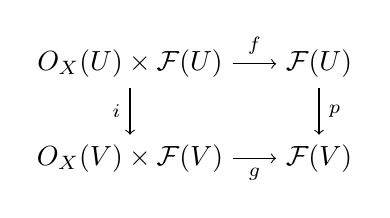
\begin{tikzpicture}[auto]
   \node (a) at (0, 1.2) {$O_X(U) \times \mathcal{F}(U)$};
   \node (x) at (2.4, 1.2) {$\mathcal{F}(U)$};
   \node (b) at (0, 0) {$O_X(V) \times \mathcal{F}(V)$};
   \node (y) at (2.4, 0) {$\mathcal{F}(V)$};
   \draw[->] (a) to node {$\scriptstyle f$} (x);
   \draw[->] (x) to node {$\scriptstyle p$} (y);
   \draw[->] (a) to node[swap] {$\scriptstyle i$} (b);
   \draw[->] (b) to node[swap] {$\scriptstyle g$} (y);
   \end{tikzpicture}
\end{itemize}
\end{dfn}
\end{screen}


この時,$\mathcal{F},\mathcal{G}$のテンソル積,$\mathcal{F} \otimes_{O_X} \mathcal{G}$を
\begin{equation*}
U \mapsto \mathcal{F}(U) \otimes_{O_X(U)} \mathcal{G}(U)
\end{equation*}
の層化したものを$\mathcal{F} \otimes_{O_X} \mathcal{G}$で表す.
また$(\mathcal{F} \otimes_{O_X} \mathcal{G})_x = \mathcal{F}_x \otimes_{O_X, x} \mathcal{G}_x$となる.
これは\ref{tensor module}で示す.


\begin{screen}
\begin{dfn}
$(X, O_X)$加群$\mathcal{F}$に対し,$\mathcal{F}$が$x \in X$でglobal sectionで生成されるとは,
\begin{equation*}
  O_{X,x} \otimes \mathcal{F}(X) \twoheadrightarrow \mathcal{F}_x
\end{equation*}
となること.
$\forall x \in X$でglobal sectionで生成される時,$\mathcal{F}$はglobal sectionで生成されるという.
$S \subset \mathcal{F}(X)$に対し,$\{s_x \mid s \in S\}$が$\mathcal{F}_x$を生成する時$S$で生成されるという.
\end{dfn}
\end{screen}

\begin{lem}
 $\mathcal{F}$がglobal sectionで生成されていることと$O_X^{(I)} \twoheadrightarrow \mathcal{F}$と同値.
\end{lem}
\begin{proof}
$O_X^{(I)} \twoheadrightarrow \mathcal{F}$ならば$\mathcal{F}$がglobal sectionで生成されていることを示す.

   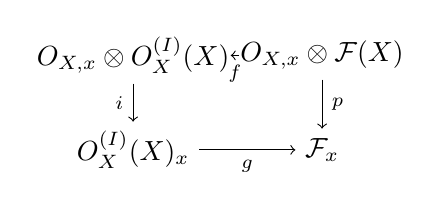
\begin{tikzpicture}[auto]
   \node (a) at (0, 1.2) {$O_{X,x} \otimes O_X^{(I)}(X) $};
   \node (x) at (2.4, 1.2) {$O_{X,x} \otimes \mathcal{F}(X)$};
   \node (b) at (0, 0) {$O_X^{(I)}(X)_x$};
   \node (y) at (2.4, 0) {$\mathcal{F}_x $};
   \draw[->] (a) to node {$\scriptstyle f$} (x);
   \draw[->] (x) to node {$\scriptstyle p$} (y);
   \draw[->] (a) to node[swap] {$\scriptstyle i$} (b);
   \draw[->] (b) to node[swap] {$\scriptstyle g$} (y);
   \end{tikzpicture}

が成り立ち,$i$は$O_X^{(I)}$は$O_X$加群としてglobal sectionで生成されているので全射.
また,$g$は仮定から全射となる.よって$p$は全射となるので,global sectionで生成されている.

逆を示す.$S$として$\mathcal{F}(X)$を取ることにより,必ず$\mathcal{F}$を生成する$S$が存在する.
また,$e_s \in O_X^S(U)$を$e_s(s) = 1, e_s(t) = 0$となる元とし,
$O_X^{S}(U) \to \mathcal{F}(U), \sum_{s \in S} a_s e_s \mapsto a_s s_U$とすれば,
これは層の間の射となり,全射性も言える.
\end{proof}


\begin{screen}
\begin{dfn}
$(X, O_X)$加群の層$\mathcal{F}$が\textbf{quasi coherent shaef}とは$\forall x \in X$に対し,$x \in U$が存在し,
\begin{equation*}
  O_X^{(J)}|_U \to O_X^{(I)}|_U \to \mathcal{F}|_U
\end{equation*}
がexactとなることを言う.
\end{dfn}
\end{screen}

\subsection{Quasi-Coherent Sheaves on an affine scheme}
$X = \mathrm{Spec}A$の時にquasi-coherent sheafを構成する.
$M$を$A$-modする.
$\tilde{M}$という$O_x$-加群を構成する.
\begin{equation*}
\tilde{M}(D(f)) := M_f = M \otimes_A A_f
\end{equation*}
とする.
$D(g) \subset D(f)$の時,$V(g) \supset V(f)$なので,
$\cup_{f \in p}p  = \sqrt{(f)} \ni g$となる.よって$g^n = fb$とかける.これより

\begin{alignat*}{2}
 A_f & \to &  \ A_g \\
 \frac{a}{f^m} & \mapsto & \ \frac{b^ma}{g^{mn}}
\end{alignat*}

が定まり,それの誘導する射

\begin{alignat*}{2}
 M_f & \to &  \ M_g \\
 \frac{x}{f^m} & \mapsto & \ \frac{b^m x}{g^{mn}}
\end{alignat*}

が定義される.
この時$\{D(f)\}$上で$\tilde{M}$が$\mathcal{B}$-sheafになることを示す.
\begin{align*}
  & X = \cup D(f_i) \\
\Leftrightarrow & X = D \left(\sum (f_i) \right) \\
\Leftrightarrow & V \left(\sum (f_i) \right) = \emptyset
\end{align*}
この時,$\sum f_i = (1)$より,$\sum a_i f_i = 1$とかける.
よって$a_i$が$0$でない$f_i$を使い,$X = \cup_{i=1}^n D(f_i)$とかける.

$X$のfinite open coveringについて,$X$について層の定義を満たすことを示せば十分である.
$X$についての条件を満たせれば,$X=D(f)$の時について示せる,それは$D(f) \cup D(f_i)$がAffineになるので,$D(f)$というスキームのfinte open coveringについて示せる.
また,finite open coverの時に言えれば,compactなのでopen coverに対し,affin finte open coverが取れ、そこ上で成り立つことを示せばよい。
特に
\subsection{Coherent sheaves}


\begin{lem}
\label{tensor module}
$X$上の$O_X$加群$\mathcal{F},\mathcal{G}$のテンソル積,$\mathcal{F} \otimes_{O_X} \mathcal{G}$を
$\mathcal{F} \otimes_{O_X} \mathcal{G}(U) := \mathcal{F}(U) \otimes_{O_X(U)} \mathcal{G}(U)$とすると層になる
また$(\mathcal{F} \otimes_{O_X} \mathcal{G})_x = \mathcal{F}_x \otimes_{O_X, x} \mathcal{G}_x$となる.
\end{lem}
環つき空間をスキームの場合に限定して示す. 局所的なので、$X$をアフィンスキームと思って良い.

\begin{lem}
$S^{-1}N \otimes M \sim S^{-1}(N \otimes M)$
\end{lem}
真面目に元をおえば示せる.


\begin{lem}
$S^{-1}(N \otimes M) \sim S^{-1}N \otimes_{S^{-1}R} S^{-1}M$
\end{lem}
これは$S^{-1}N = N \otimes S^{-1}R$より
\begin{equation*}
  S^{-1}N \otimes_{S^{-1}R} S^{-1}M \sim N \otimes S^{-1}R \otimes_{S^{-1}R} S^{-1}M \sim N \otimes S^{-1}M \sim  S^{-1}(N \otimes M)
\end{equation*}
となる.

これを使うことにより,スキームに対しては成り立つことがわかる.
おそらく,一般の場合は上と近い形で
$O(V) \otimes_{O(U)} M(U) \otimes N(V) \to M(V) \otimes N(V)$と
$N(U) \otimes M(U) \to O(V) \otimes N(U) \otimes M(V)$とを使いながら,これのらindcutive limitが一致することを示せばよいはず。


\end{document}
